\chapter{Introduction}
\label{ch:introduction}

\begin{quotation}[Um Passeio No Mundo Livre, Afrociberdelia]{Chico Science}
Um passo a frente e você não está mais no mesmo lugar\\
One step forward and you are not in the same place
\end{quotation}

Software maintenance and evolution are characterised by their huge cost and
slow speed of implementation. However they are inevitable activities -- almost
all software that is useful and successful stimulates user-generated requests for
change and improvements \citep{Bennett2000}. Sommerville
\citep{Sommerville2007} is even more emphatic and says that software changes
is a fact of life for large software systems. In addition, a set of studies
\citep{Huff1990,Moad1990,Eastwood1993,Erlikh2000} has stated along the years
that software maintenance and evolution is the most expensive phase of
software development, taking up to 90\% of the total costs.

All of these characteristics from software maintenance leaded the academia and
industry to investigate constantly new solutions to reduce costs in such
phase. In this context, \acf{SCM} is a set of
activities and standards for managing and evolving software, defining how to
record and process the proposed system changes, how to relate these to system
components, among other procedures. For all these tasks, it has proposed
different tools, such as version control systems and bug trackers
\citep{Sommerville2007}. However, some issues may arise due to these tools
usage. In this work, the focus are the issues from bug trackers, as
it will be discussed along this dissertation.

The remainder of this chapter describes the focus of this dissertation and
starts by presenting its motivation in \secref{sc:motivation} and a clear
definition of the problem in \secref{sc:problem}. An overview of the proposed
solution is presented in \secref{sc:solution}, while \secref{sc:outofscope}
describes some related aspects that are not directly addressed by this work.
\secref{sc:contributions} presents the main contributions and, finally,
\secref{sc:structure} describes how this dissertation is organized.


\section{Motivation}
\label{sc:motivation}
Aiming to improve change management processes, some organizations have used
specific systems (generally called \emph{bug-trackers}) to manage, store and
handle change requests (also known as \emph{bug reports}). A bug report is
defined as a software artifact that describes some defect, enhancement, change
request, or an issue in general, that is submitted to a bug tracker;
generally, bug report submitters are developers, users, or testers. Such
systems are useful because changes to be made in a software can be quickly
identified and submitted to the appropriate people \citep{Anvik2005}.

Moreover, the use of bug trackers helps to monitor the software evolution,
because bug reports are recorded in a database as well as people involved
in a particular bug report are recorded. Thus, changes and their respective
responsible can be easily found. Organizations also use such systems to guide
the development of software, thus any task to be undertaken in the software
development process must be registered and monitored through a bug-tracker. In
addition, the historical data of these systems can be used as history and
documentation for the software. Examples of such systems are
Bugzilla (\url{http://www.bugzilla.org}), Mantis (\url{http://www.mantisbt.org})
and Trac (\url{http://trac.edgewall.org}).

Each bug report is stored with a variety of fields of free text and custom
fields defined according to the necessity of each project. In Trac, for
example, it is defined fields for summary and detailed description of a
bug report. In the same bug report it can also be recorded information about
software version, dependencies with other bug reports (duplicate bug reports,
for example), the person who will be assigned to the bug report, among other
information. Moreover, during the life cycle of a bug report, comments can
be inserted to help solving it. Figure \ref{fg:tracbug} shows an example of a
bug report from Trac.

%\usepackage{graphics} is needed for \includegraphics
\begin{figure}[htp]
\centering
  \fbox{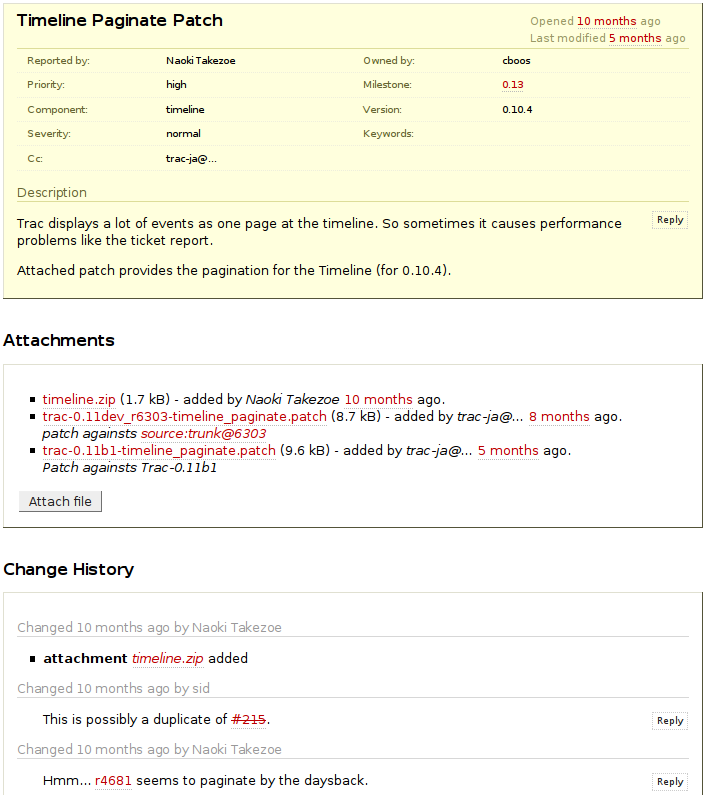
\includegraphics[width=\textwidth]{chapters/introduction/tracbug.png}}
  \caption[Example of a bug report]{Example of a bug report}
  \label{fg:tracbug}
\end{figure}

Some challenges have emerged through the use of bug trackers,
among them, we can cite: dynamic assignment of bug reports \citep{Anvik2006a},
change impact analysis and effort estimation \citep{Song2006}, quality of bug
report descriptions \citep{Ko2006}, software evolution and traceability
\citep{Sandusky2004}, and duplicate bug reports detection \citep{Hiew2006}.
Each one of these issues are briefly described as follows:

\begin{itemize}
  \item \textbf{Dynamic assignment} of bug reports is to detect (automatic or
semi-automatically) the best developer suited to solve a problem reported
in a bug report;
  \item \textbf{Change impact analysis} and \textbf{effort estimation}
focus on calculating the impact of a bug report in a project and calculating the
necessary effort to solve it;
  \item \textbf{Quality of bug report descriptions} is to ensure that the
  submitted bug reports are properly described;
  \item \textbf{Software evolution traceability} is concerned with
the understanding what drives the changes performed in the software along the
time; and
  \item \textbf{Duplicate bug reports detection} consists in avoiding the
  submission of bug reports that describe an already submitted issue.
\end{itemize}

The focus of this work is trying to avoid duplicate bug reports submission. The
problem of bug reports duplication is better explained and characterized in
Chapter 4, through a study which examines the factors that cause
it and how it impacts on the software development. Furthermore, the other
challenges are further detailed on Chapter 3, where it is
described the state-of-the-art of mining bug report repositories.

\section{Problem Statement}
\label{sc:problem}
The goal of this dissertation can be stated as follows:

\begin{quote}
\emph{This work investigates the problem of bug report duplication emerged
by bug trackers, characterizing it empirically to understand its causes and
consequences, and provides a tool for search and analysis of bug reports to
reduce the effort spent on such tasks.}
\end{quote}

\section{Overview of the Proposed Solution}
\label{sc:solution}
In order to reduce the effects of the bug report duplication problem, it was
developed the \acf{BAST}. The remainder of this section describes the context
where it was developed and the outline of the proposal.

\subsection{Context}
This dissertation is part of the \ac{RiSE} \citep{Almeida2004}, formerly
called RiSE Project, whose goal is to develop a robust framework for software
reuse in order to enable the adoption of a reuse program. However, it is
influenced by a series of areas, such as software measurement, architecture,
quality, environments and tools, and so on, in order to achieve its goal. The
influence areas are depicted in \figref{fg:rise-spiral}.

%\usepackage{graphics} is needed for \includegraphics
\begin{figure}[htp]
\begin{center}
  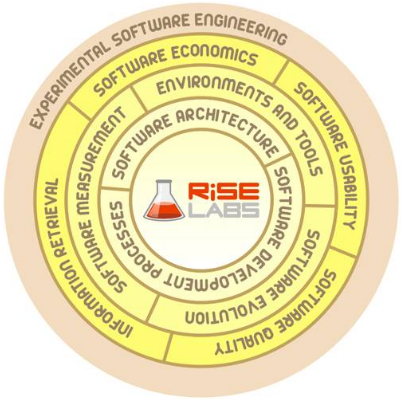
\includegraphics[width=9cm]{chapters/introduction/rise-spiral.png}
  \caption[RiSE Labs Influences]{RiSE Labs Influences}
  \label{fg:rise-spiral}
\end{center}
\end{figure}

Based on these areas, the RiSE Labs is divided in several projects, as shown in
Figure \ref{fg:rise-projects}. As it can be seen, this framework embraces
several different projects related to software reuse and software engineering.
They are:

\begin{itemize}
  \item \textbf{RiSE Framework:} Involves reuse processes
  \citep{Almeida2004,Nascimento2008}, component certification
  \citep{Alvaro2006} and reuse adoption process \citep{Garcia2008a}.
  
   \item \textbf{RiSE Tools:} Research focused on software reuse tools, such
   as the Admire Envi- ronment \citep{Mascena2006}, the Basic Asset Retrieval
   Tool (B.A.R.T) \citep{Santos2006}, which was enhanced with folksonomy
   mechanisms \citep{Vanderlei2007}, semantic layer \citep{Durao2008},
   facets \citep{Mendes2008} and data mining \citep{Martins2008}, and the
   Legacy InFormation retrieval Tool (LIFT) \citep{Brito2007};
   
   \item \textbf{RiPLE:} Development of a methodology for Software Product
   Lines \citep{Filho2008};
   
   \item \textbf{SOPLE:} Development of a methodology for Software Product
   Lines based on services;
   
   \item \textbf{MATRIX:} Investigates the area of measurement in reuse and
   its impact on quality and productivity;
   
   \item \textbf{BTT:} Research focused on tools for detection of duplicate
   bug reports, such as in \citet{CavalcantiFISL2008}. Thus, this work is part
   of the BTT research group;
   
   \item \textbf{Exploratory Research:} Investigates new research directions
   in software engineer- ing and its impact on reuse;

   \item \textbf{CX-Ray:} Focused on understanding the \ac{C.E.S.A.R.}, and its
   processes and practices in software development.
\end{itemize}

This dissertation is part of the \ac{BTT} project and its goal is to
provide a tool for search and analysis of bug reports with the objective of
avoiding duplicate bug reports submission. This work was conducted inside a
group for software reuse research, because the bug report duplication problem
is more prone to appear when different parts of software are being reused by
different projects. A common case where software reuse implies the submission
of duplicate bug reports is when the concept of Software Product Lines
\citep{Pohl2005} approach is used to develop software \citep{Runeson2007}. In
this context, different software projects share the same basis components, and
if some of these components are defective they will affect all software that
use these components, thus increasing the possibility of duplicate bug
reports submission.

\begin{figure}[htp]
\begin{center}
  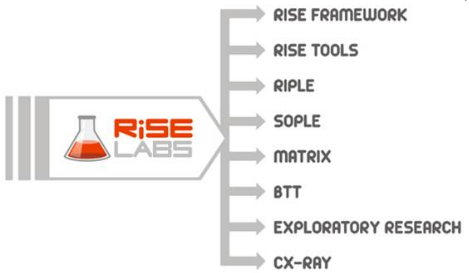
\includegraphics[width=10cm]{chapters/introduction/rise-projects.png}
  \caption[RiSE Labs Projects]{RiSE Labs Projects}
  \label{fg:rise-projects}
\end{center}
\end{figure}

\subsection{Outline of the Proposal}
The proposed solution consists in a Web based application that enables people
involved with bug report search and analysis to perform such tasks
more effectively. Although bug report tracking process involves a complete
cycle of finding errors, reporting them, validating, fixing the problems and, finally,
releasing the changes, the proposed solution aims to assess only the reporting
phase. However, the benefits of improving the reporting phase of bug tracking
can be reflected to the other phases also, since the time that is saved
in the reporting phase can be used to perform the tasks involved in other
phases.

\section{Out of Scope}
\label{sc:outofscope}

\begin{itemize}
  \item \textbf{Quality of search results.} The proposed solution uses a
  well-known model (Vector Space Model \citep{Salton1975}) to represent
  documents and perform searches that better meets our necessity, however it
  is out of the scope of this work to analyze how efficient is the model. Some
  discussion involving the efficiency of this model can be found in the work
  of \citet{Salton1975};
  
  \item \textbf{Impact on other phases of bug tracking process.} Our solution
  concerns with the reporting phase from bug tracking process. Thus, we are
  interested on how this phase can be improved by the proposed solution. In this
  way, it is out of scope the analysis and improvement of other phases;
  
  \item \textbf{Type of users.} Initially, the subjects of this work can be
  developers, testers or other stakeholders with some technical background in
  software development, specially using bug trackers. Thus, it is out of scope
  to provide a tool that supports all types of users.
\end{itemize}

\section{Statement of the Contributions}
\label{sc:contributions}
As a result of the work presented in this dissertation, the following
contributions can be highlighted:

\textbf{A characterization of the bug report duplication problem.} It was
conducted an extensive study about the duplication problem in order to confirm
its existence, and potential causes for bug report duplication.

\textbf{An analysis of the state-of-the-art for mining bug report repositories.}
It presents an overview of the work found in the literature that have
mined specifically bug report repositories, for all diverse purposes.

\textbf{A solution for bug reports duplication.} It specifies and
implements a solution based on \emph{Text Mining} and \emph{Keyword search}
techniques \citep{Baeza1999}, with the objective of to reduce the effects of
the bug report duplication problem.

\textbf{Two empirical studies to validate the proposed solution.} This
dissertation also presents a case study performed in a real environment for
software development and test, and an experiment performed with 18 subjects
comparing \ac{BAST} with a baseline tool.

In addition to the contribution mentioned, some papers presenting the
findings of this dissertation were produced:

\begin{itemize}
  \item Cavalcanti, Y. C., Martins, A. C., de Almeida, E. S., and de Lemos
  Meira, S. R. (2008a). Avoiding Duplicate CR reports in Open Source Software
  Projects. In \emph{The 9th International Free Software Forum (IFSF'08)}, Porto
  Alegre, Brazil.
  
  \item Cavalcanti, Y. C., de Almeida, E. S., da Cunha, C. E. A., Pinto, E. R.,
  and Meira, S. R. L. (2008b). The Bug Report Duplication Problem: A
  Characterization Study. Technical report, C.E.S.A.R and Federal University
  of Pernambuco.
\end{itemize}

\section{Example of Listings Package}
\lstset{language=C,basicstyle=\small}
\begin{lstlisting}[caption=This is a simple use of listings package.]
#include <stdio.h>
#define N 10
/* Block
 * comment */
 
int main() {
    int i;
    // Line comment.
    puts("Hello world!");
    for (i = 0; i < N; i++) {
        puts("LaTeX is also great for programmers!");
    }
    return 0;
}
\end{lstlisting}
